\subsection{Feature Module: Generating View Descriptors}
\label{sec:architecture-feature-module}
The objective of the feature module is the generation of a descriptor for each view by using five convolutional layers.
Each one is referred to as a view descriptor $\vec{V}_i$ in the following.
\figref{fig:feature-module} shows the basic concept.
\begin{figure}
	\centering
	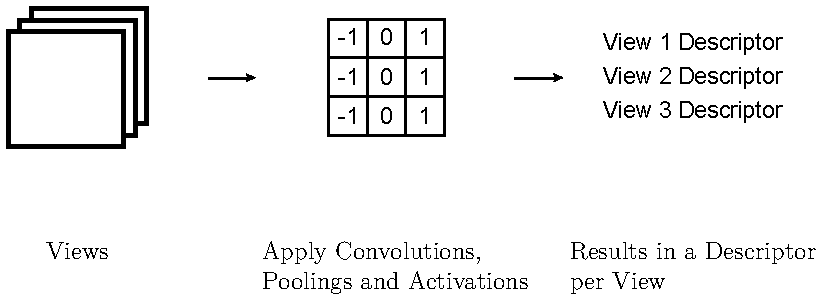
\includegraphics[]{images/feature_module.pdf}
	\caption{Basic Concept of the Feature Module}
	\label{fig:feature-module}
\end{figure}
This module is the first one in the feed-forward chain.
It is connected with the real world by having all views $\mathbb{V}$ of an object as its input.
Furthermore, because tensorflow supports batch execution, i.e. all its operations can be applied to a batch of data, the input tensor is extended with a batch dimension for multiple multi-views.
This yields an input tensor of shape $Batch \times Views \times Height \times Width \times Channels$.
In the following, if a tensor has a batch dimension, which is usually the case, it is assumed that any mentioned operation or approach is applied to every batch element.
This module consists of five main convolutional layers.
A main convolutional layer is supposed to have a convolutional layer and an optional pooling layer.
The first main layer performs a valid convolution with 96 filters of size $7 \times 7$ and a stride of 2 on each $224 \times 224 \times 3$ input.
Every filter extracts different features.
In comparison, the original AlexNet uses filters of size $11 \times 11$ and a stride of 4.
However, it is assumed that smaller filters and a smaller stride are collecting more information that can be used for a classification of the object and material at once.
A convolution operation is done by flattening the filter tensor to a 2D matrix of size $Filter\_Height \times Filter\_Width \times Channels\_In \times Channels\_Out$.
Here, $Channels\_in = 3$ because of the RGB channels of the input image and $Channels\_Out = 96$ because of the defined number of filters.
Then, image patches of shape $Batch \times Height\_Out \times Width\_Out \times Filter\_Height \cdot Filter\_Width \cdot Channels\_In$ are extracted from the input tensor.
Multiplying the filter matrix and the image patch vector yields the convolution results for the current window.
This is repeated for the whole input resulting in a matrix with a size of $1 \times 109 \times 109 \times 96$ in this case.
Furthermore, to each convolution output the corresponding bias is added.
This result is fed into a ReLU activation function.
Finally, the outputs are max-pooled with a window of size $3 \times 3$ and a stride of 2.
No padding is applied as well.
It is defined, that the max-pooling is always performed on the last dimension, i. e. the one containing each feature.
This yields a matrix of shape $1 \times 54 \times 54 \times 96$ for each convolution.
The next layers are similar including the bias addition and the ReLU activation function.
Hence, only the operations and their parameters will be mentioned.
Furthermore, the layers are added sequentially.
That means, the activations of the previous main layer are the input of the current main layer and so on.
The second main layer performs a convolution with 256 filters of size $5 \times 5$ and a stride of 2.
However, this time the input is padded in a way, that the output has the original input's size.
This yields a convolution result of shape $1 \times 27 \times 27 \times 256$.
The max-pooling uses again a window of $3 \times 3$ and a stride of 2.
The valid padding technique is applied resulting in a shape of $1 \times 13 \times 13 \times 256$.
The third and fourth main layer use 384 filters of size $3 \times 3$ for the convolution task with a stride of 1 each and the padding technique same.
However, no pooling is performed.
Hence, this yields a matrix of shape $1 \times 13 \times 13 \times 384$ both the times.
For the last main layer, the fifth one, a convolution with 256 filters of size $3 \times 3$ is performed.
The stride is 1 and the padding technique same, hence, the result has a size of $1 \times 13 \times 13 \times 256$.
The output's dimension is reduced with a valid max-pooling of size $3 \times 3$ and a stride of 2 to $1 \times 6 \times 6 \times 256$.
In the end, this whole process results in a tensor containing each view descriptor $\vec{V}_i$ of size $6 \times 6 \times 256$ of every batch element.
Hence, this tensor's shape is $Batch \times Views \times 6 \times 6 \times 256$.